\chapter{Technical Background}
\section{SHAMPU}
SHAMPU\cite{smeets2014demonstration} is a design framework which allows remote debugging and reprogramming of sensor nodes. Its main advantages over other testbeds (see section~\ref{sec:related_work}) are portability, low cost, small size and low energy consumption. SHAMPU is used as an extension to an already existing sensor node. The only requirement is that the node provides an USB-Interface which is connected to SHAMPU. This single connection to the attached node makes SHAMPU OS independent.
\begin{figure}[H]
	\centering
	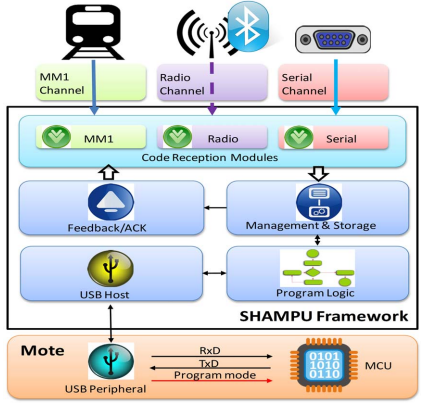
\includegraphics[scale=.5]{content/images/SHAMPUframework.png}
	\caption{Overview of the SHAMPU Framework \cite{smeets2014demonstration}}\label{fig:shampuframework}
\end{figure}
The SHAMPU framework (see Figure \ref{fig:shampuframework}) itself is split into multiple modules. The most important part for this thesis is the Code Reception Module, which allows the use of different protocols to connect to and communicate with the SHAMPU device. One option for the wireless communication with a SHAMPU device is the ANT protocol, on which we will focus in this evaluation.

\section{ANT}
ANT \cite{DynastreamInnovationsInc.2013} is a wireless protocol which operates in the 2.4 GHz ISM Band. It was originally developed in 2003 by Dynastream Innovations Inc. for the use in wireless sensors. The ANT protocol is designed for the use in low power WSNs, focusing on small size and ease of use.

One of the advantages ANT has over other protocols, such as Bluetooth or ZigBee, is the high level of abstraction the ANT Protocol provides. 
\begin{figure}[H]
	\centering
	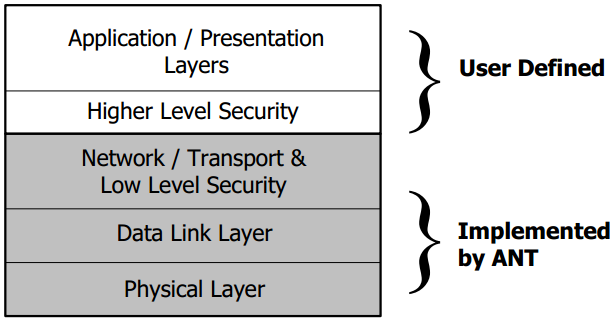
\includegraphics[scale=.5]{content/images/ANTstack.png}
	\caption{OSI-Layer vs. ANT Protocol\cite{Networks}}\label{fig:osilayer}
\end{figure}

This level of abstraction is achieved by incorporating the first 4 OSI-layers (see Figure \ref{fig:osilayer}) into the ANT protocol, thus allowing even low-cost microcontrollers to set up and maintain complex wireless networks, since all the details of the communication are handled by the ANT-chip.

\subsection{ANT Topology}
In order for the ANT protocol to work each mote needs to be part of a network. As shown in figure \ref{fig:anttopo} the ANT protocol can be used to create simple or considerably more complex networks. Each mote inside a network is called an ANT node. In order for two nodes to communicate with each other they need to be connected via a channel.

\begin{figure}[H]
	\centering
	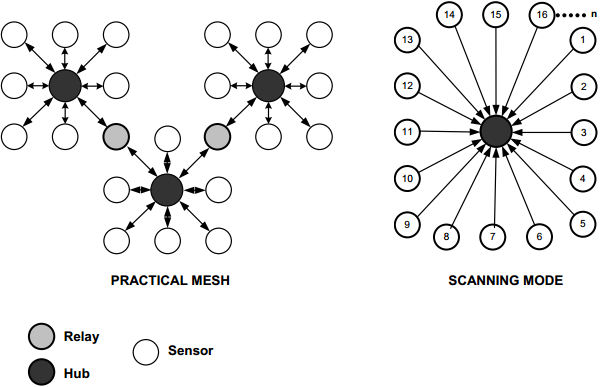
\includegraphics[scale=0.7]{content/images/ANTtopo.png}
	\caption{Example ANT Topologies\cite{DynastreamInnovationsInc.2013}}\label{fig:anttopo}
\end{figure}

\subsection{ANT Channels}
\label{sec:ANTchan}
The ANT protocol uses virtual channels to allow different nodes to transmit data, without interfering with each other. Each channel can be assigned to a 1 MHz wide RF frequency band between 2400 MHz and 2524 MHz.\cite{DynastreamInnovationsInc.2013} In theory this allows 125 different channels to exist without interference between them. It is possible for multiple channels to use the same frequency depending on the rate of transmission, since the data rate of each 1MHz band is limited to 1MBps. 
To avoid interference between nodes which use the same frequency isochronous self adjusting Time Division Multiple Access (TDMA) is used. TDMA allows the ANT protocol to adjust the transmit timings of the channels individually.

Each node has to specify how the assigned channel is being used. The node can either be a master or a slave node. While a master node mostly sends data and a slave node mostly receives data, the slave retains the ability to respond to the incoming data.

The ANT protocol further differentiates between two different channel types:
\begin{description}
	\item{\textbf{Independent Channels}} \hfill \\ Independent Channels are used if there is only one node which transmits data. There is no limit to the amount of slave devices which receive messages. Furthermore, the message being sent out is broadcast to all nodes. Tt is not possible to address only a specific node.
	\item{\textbf{Shared Channels}} \hfill \\ Shared Channels are used if there is more than one node which sends data. This type of channel is facilitated by the use of a Shared Channel Address, which in turn reduces the amount of data that can be transmitted at a time. All ANT nodes still receive every message, but only pass on messages which have a matching address. The Channel master can decide to either use one or two bytes as the address, which allows for either 255 or 65535 slave devices in the same channel. 
\end{description}

\begin{figure}[H]
	\centering
	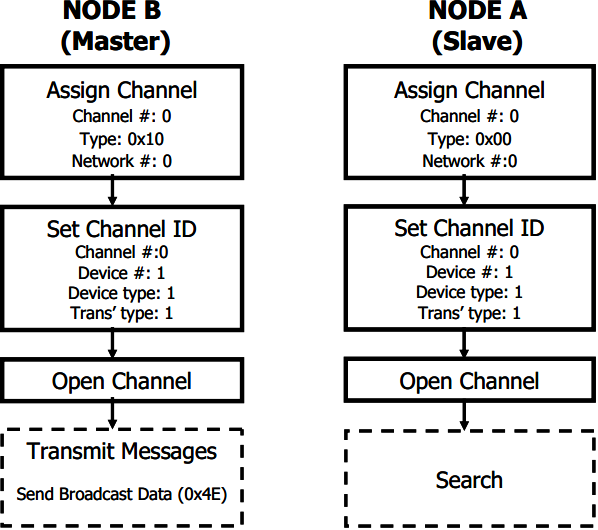
\includegraphics[scale=0.7]{content/images/ANTsetup.png}
	\caption{ANT channel establishment\cite{DynastreamInnovationsInc.2013}}\label{fig:antsetup}
\end{figure}

Figure \ref{fig:antsetup} shows the procedure of opening up a channel between two ANT nodes. In the first step the channel configuration is set, most important in this context being the channel type: 0x00 signifies that the node is opening the channel as a slave while 0x10 means that the node acts as a master. The next step is to set the Channel ID. Since it is possible for two nodes to transmit on the same frequency, the device number, device type and transmission type of the slave node need to match the values of the master it wants to connect to. It is possible, however, to set wild card values, which allows the slave to connect to any device sending on the same frequency. Before the final step, it is optionally possible to set the frequency of the channel, the power setting and the message period. These steps are not mandatory though, since ANT defaults to fixed values: 2466 Hz transmission frequency, 0dBm power and a message period of 8192. The last step constitutes of the opening of the channel itself. The master should open the channel before the slave to ensure a successful connection.

\subsection{ANT Communication}

The ANT protocol supports three different data types: broadcast, acknowledge and burst. The data type is not part of the channel configuration, thus channels are able to use any combination of data types. The only exceptions are legacy unidirectional channels, which can only send broadcast data. The various data types differ in the way data is handled and transmitted.
\begin{figure}[H]
	\centering
	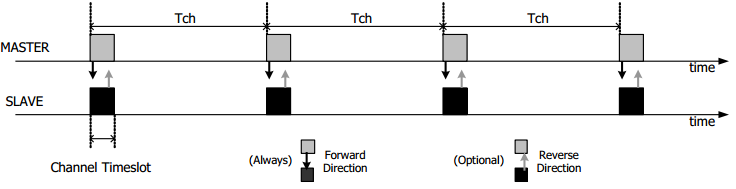
\includegraphics[scale=.75]{content/images/ANTdataflow.png}
	\caption{ANT channel communication \cite{DynastreamInnovationsInc.2013}}\label{fig:antflow}
\end{figure}

\begin{itemize}
	\item{Broadcast data} \hfill \\ Broadcast data represents the most basic data type and, at the same time, the default. To start a broadcast transmission, the command needs to be issued just once, since the last sent packet is continuously resent as a broadcast. It does not matter whether the last packet was part of a burst or acknowledge transmission. If no new data is available this packet is resent. Figure \ref{fig:antflow} shows, how each broadcast transmission is aligned to the channel with a message period $T_{ch}$. Since there is no answer from the receiving node, it is not possible to determine if the packet was transmitted correctly.
	
	\item{Acknowledge data} \hfill \\ Acknowledge data can be used to ensure a node has received a transmitted packet. After receiving an acknowledge packet the node will send a message back to the sender. Acknowledge data should only be used as a unicast, since if multiple nodes send an acknowledge message back, the messages can interfere with each other. Figure \ref{fig:antflow} shows that, just like broadcast data, acknowledge data is always aligned to a time slot, yet the receiver does not wait for the next time slot and instead sends the answer immediately back to the sender.
	
	\item{Burst data} \hfill \\ Burst data provides a method to quickly transmit larger amounts of data. This is achieved by ignoring the normal channel time slots and sending the packets immediately one after the other. This allows for a transmission rate of up to 20 kbps \cite{DynastreamInnovationsInc.2013}, which is much higher than the other data transmission types. Similar to acknowledge data at the end of the transmission the sender is informed whether the transfer failed or succeeded. Just like acknowledge data, burst transmission should be unicast, since if one node fails to receive a packet the transmission is stopped. The drawback of this method is, that burst data is prioritized over all other transmissions and will interrupt other transmissions over the same RF frequency.
\end{itemize}

\subsection{ANT messages}
In the ANT protocol each message has the basic format as specified in Figure \ref{fig:antmsg}.
\begin{figure}[H]
	\centering
	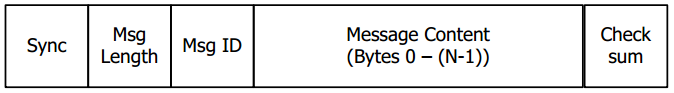
\includegraphics[scale=.75]{content/images/ANTmsg.png}
	\caption{ANT message structure\cite{DynastreamInnovationsInc.2013}}\label{fig:antmsg}
\end{figure}
Each message starts with a special Sync-Byte and ends with a checksum, which is calculated by xoring all previous bytes. The Msg Length byte shows the number of Message Content bytes. The Msg ID byte specifies which kind of data is contained in the message. The ANT protocol also provides an extended message format, which allows to attach further information to each message. The length of the message varies between message types, but the size of the payload for each of the three different data-transmission types is always at 8 bytes.

\section{ANT library}
There is an official ANT library \cite{ANTWinLib} available, however this library is written in C++ for Windows. Since SHAMPU uses a PIC24FJ64GB002 microcontroller\cite{smeets2014demonstration} it is not possible to use the official library. Instead we use an already existing ANT library for this thesis \cite{ANTPICLIB}. This library implements almost the complete ANT API, except for two important features. The library uses busy-waiting to receive packets. Also sending burst transmission does not work correctly. In order to be able to use ANT efficiently with SHAMPU we implemented a non-blocking packet receiver. This is an important addition to the code, because otherwise the microcontroller is not able to function, while it is waiting for a packet. Unfortunately we were not able to get burst mode working correctly. Burst packets need to have a precise timing, but the black box nature of the ANT protocol makes it a challenge to debug the code.
\section{ANTAP1MxIB RF}
Each SHAMPU device is equipped with an ANTAP1MxIB RF Transceiver Module\cite{Networks}. The module was chosen because of its small form factor (20mm x 20mm) and its very low power draw. The ANTAP1M can handle up to 4 different ANT channels with a combined message rate of 200 Hz. 

\begin{figure}[H]
	\centering
	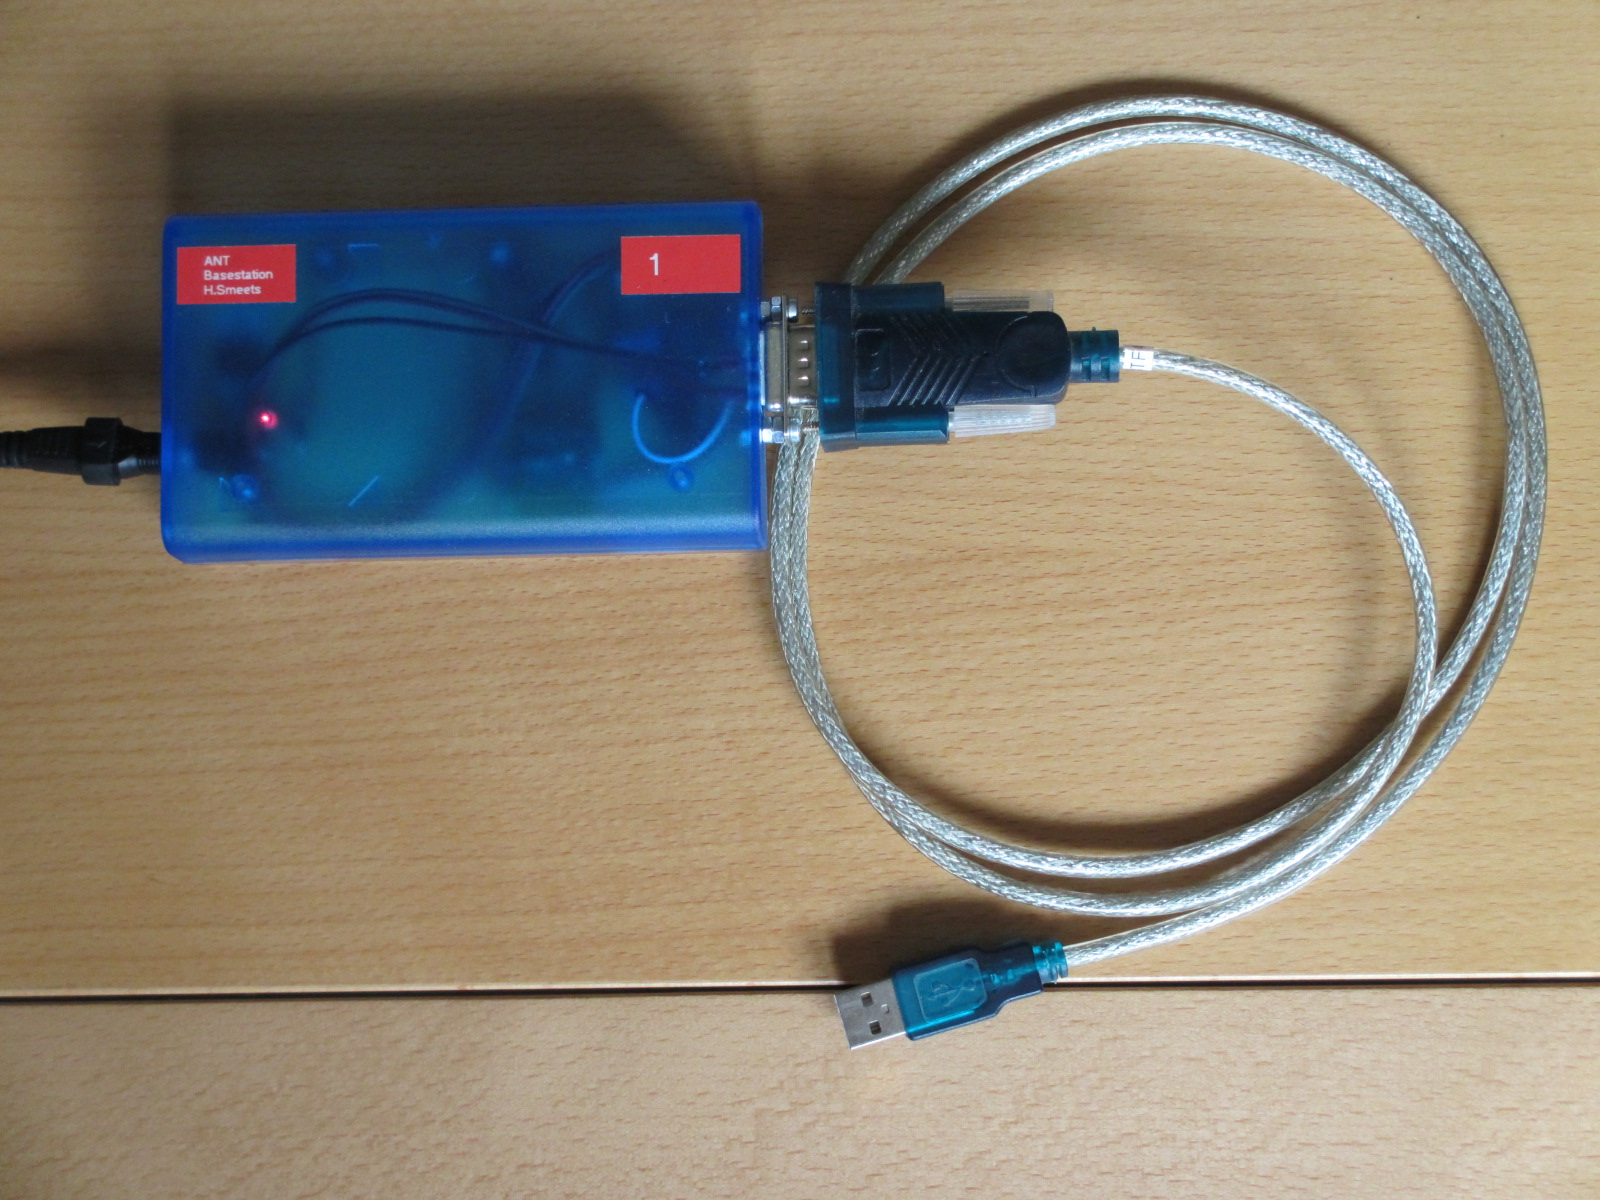
\includegraphics[scale=.5]{content/images/SHAMPUbase.JPG}
	\caption{SHAMPU base station}\label{fig:shampubase}
\end{figure}
In order to test the capabilities of the ANT chip, we used two SHAMPU base stations for all the experiments. This base station (see Figure \ref{fig:shampubase}) contains the ANTAP1MxIB and a MAX3224CPP microcontroller acting as an UART to serial interface, which allows the ANT to asynchronously communicate with a PC over RS-232. A transmission speed of 19200 baud is used which allows a data rate of 1920 Bps, since the RS-232 protocol adds a start and stop bit to each transmitted byte\cite{RS232}.
